\chapter{Resultados}

Os resultados esperados, delineados no plano de atividades \citeonline{PlanoAtividades}, foram atingidos de maneira adequada durante a execução do trabalho, para mais informações aceesar este diretório \cite{gitwotpy:readme}. A seguir, são descritos os desfechos alcançados:

\textbf{Entendimento aprofundado das especificações do W3C-WoT}: Uma análise completa das especificações do W3C-WoT foi realizada, gerando um entendimento detalhado dos conceitos e requisitos principais para a execução do WoTPy. Isso habilitou a implementação correta e eficaz do \textit{gateway}, seguindo as normas definidas pelo consórcio.

\textbf{Escolha e domínio de bibliotecas e ferramentas adequadas}: As bibliotecas e ferramentas mais apropriadas para o desenvolvimento do WoTPy foram escolhidas, considerando a compatibilidade com os protocolos de comunicação necessários e a facilidade de integração com outros projetos IoT. O domínio dessas ferramentas foi essencial para o êxito do trabalho.

\textbf{Resolução dos problemas de instalação do WoTPy}: Problemas relacionados à instalação do WoTPy foram identificados e solucionados, resultando em um processo simplificado e eficaz para implantar e configurar o \textit{gateway} em diferentes ambientes e sistemas operacionais. Isso simplificou a adoção do WoTPy por parte dos desenvolvedores e usuários finais, assegurando uma experiência mais suave.

\textbf{Confirmação das contribuições por meio de testes}: Uma série completa de testes foi conduzida para confirmar as contribuições feitas ao WoTPy. Esses testes garantiram a qualidade e a funcionalidade do \textit{gateway}, comprovando sua conformidade com os requisitos e sua capacidade de lidar com diferentes casos de uso.

\textbf{Criação de exemplos de uso e documentação}: Foi desenvolvido um exemplo prático de uso do WoTPy, demonstrando sua aplicabilidade em cenários de IoT. Além disso, uma documentação foi produzida, oferecendo orientações claras e recursos adicionais para facilitar a execução do WoTPy em projetos IoT. Isso contribuiu para a disseminação e adoção do \textit{gateway} pela comunidade.

\section{Especificações do W3C-WoT}

A Web das Coisas (WoT) é um esforço do World Wide Web Consortium (W3C) para estabelecer uma estrutura para conectar dispositivos e serviços na Internet das Coisas (IoT). O objetivo do WoT é possibilitar a interoperabilidade entre esses dispositivos, facilitando a comunicação e a integração padronizadas.

O W3C criou várias especificações que abordam diferentes aspectos do WoT. Essas especificações são essenciais para a execução e adoção do WoT, oferecendo diretrizes para descrever as características das Coisas (\textit{Things}), definir interfaces de rede, realizar a descoberta de Coisas, implementar a lógica de aplicação e assegurar a segurança e a privacidade dos sistemas WoT.

\begin{itemize}
\item Descrição de Coisas (\textit{Thing Description}) \citeonline{TD}: estabelece um formato de dados interpretável por máquinas para descrever os metadados e as interfaces de rede das Coisas. Ela fornece uma base sólida para a interoperabilidade entre as Coisas e a Web.
\item Modelos de Vinculação (\textit{Binding Templates}) \citeonline{WoTBinding}: dão orientações sobre como definir interfaces de rede em Coisas para protocolos específicos e ecossistemas de IoT. Esses modelos são úteis para assegurar a compatibilidade e a integração de diferentes sistemas.
\item Descoberta WoT (\textit{WoT Discovery}) \citeonline{WoTDiscovery}: estabelece um mecanismo para distribuição de metadados das Coisas. Ela permite a localização e acesso a informações detalhadas sobre as Coisas, facilitando a descoberta e integração de dispositivos na rede.
\item Modelos de Vinculação (\textit{Scripting API}) \citeonline{WoTScripting}: permitem a implementação da lógica de aplicação das Coisas utilizando uma API JavaScript comum. Isso simplifica o desenvolvimento de aplicativos IoT e promove a portabilidade entre fornecedores e dispositivos.
\item Diretrizes de Segurança e Privacidade (\textit{Security and Privacy Guidelines}) \citeonline{WoTSecurity}: oferecem orientações para a implementação segura das Coisas e discutem questões relacionadas à segurança e à privacidade nos sistemas WoT. Essas diretrizes são importantes para proteger os dispositivos e os dados sensíveis envolvidos nas redes WoT.
\end{itemize}

\subsection{Descrição de Coisas}

A Descrição de Coisas representa um formato de dados que pode ser interpretado por máquinas, projetado para esclarecer os metadados e as interfaces de rede das Coisas na Web das Coisas. Esta norma, formulada pelo W3C, constitui uma base firme para incentivar a interoperabilidade entre as Coisas e a Web.

A Descrição de Coisas possibilita a descrição das características, propriedades, funcionalidades e interfaces de uma Coisa de maneira estruturada e padronizada. Essa descrição abrange informações detalhadas sobre como interagir com a Coisa, acessar seus recursos e interpretar os dados que ela disponibiliza.

O uso da Descrição de Coisas facilita a compreensão das capacidades e requisitos de uma Coisa específica por diferentes dispositivos e sistemas. Isso permite a criação de aplicações e serviços que podem interagir com uma vasta gama de Coisas de maneira transparente, independentemente do fabricante ou da tecnologia subjacente.

\subsection{Modelos de Vinculação}

Os Modelos de Vinculação fornecem orientações que detalham como definir interfaces de rede em Coisas para protocolos específicos e ecossistemas de IoT. Estes modelos são essenciais para garantir a compatibilidade e integração entre diferentes sistemas.

Cada protocolo de comunicação usado na Web das Coisas possui suas próprias especificidades e requisitos. Os Modelos de Vinculação fornecem um conjunto de instruções e recomendações para mapear funcionalidades e recursos de uma Coisa em um formato compatível com um protocolo específico.

Ao utilizar os Modelos de Vinculação, é possível cirar interfaces de rede para as Coisas que estejam em conformidade com os requisitos e padrões dos protocolos específicos. Isso facilita a comunicação e interação entre as Coisas e os sistemas que usam esses protocolos, garantindo maior interoperabilidade e uma integração mais harmoniosa.

Além disso, os Modelos de Vinculação ajudam a promover a reutilização de código e a padronização na implementação de interfaces de rede. Ao seguir estas orientações, é possível garantir que as Coisas sejam facilmente integradas em ecossistemas IoT existentes, evitando a necessidade de desenvolver soluções customizadas para cada protocolo.

A utilização dos Modelos de Vinculação também contribui para a escalabilidade e a flexibilidade dos sistemas IoT. Como esses modelos oferecem uma estrutura padronizada para a definição de interfaces de rede, é mais fácil adicionar novas Coisas ao ecossistema e integrá-las com os sistemas existentes, o que facilita a expansão dos ecossistemas IoT e o desenvolvimento de soluções mais amplas e interconectadas.

\subsection{Descoberta WoT}

A Descoberta WoT é um mecanismo que estabelece a distribuição de metadados das Coisas na Web das Coisas. Esta norma, desenvolvida pelo W3C, possibilita a localização e o acesso a informações detalhadas sobre as Coisas, facilitando a descoberta e a integração de dispositivos na rede.

A Descoberta WoT é crucial na Web das Coisas, pois permite que os dispositivos IoT sejam descobertos e identificados de maneira eficaz. Isso é especialmente importante em ambientes onde há uma grande quantidade de Coisas interconectadas, tornando a descoberta manual desses dispositivos impraticável.

Ao utilizar o mecanismo de Descoberta WoT, é possível adquirir metadados sobre as Coisas, como suas funcionalidades, propriedades, interfaces de rede e outros atributos relevantes. Essas informações detalhadas permitem que os desenvolvedores e os sistemas IoT identifiquem as Coisas que são relevantes para suas necessidades específicas.

Além disso, a Descoberta WoT permite a integração de dispositivos de diferentes fabricantes e tecnologias. Através da distribuição de metadados padronizados, os sistemas IoT podem identificar e interagir com as Coisas de maneira consistente, independentemente de suas características individuais.

A Descoberta WoT também contribui para a escalabilidade e flexibilidade dos sistemas IoT. Com a capacidade de localizar e acessar informações detalhadas sobre as Coisas, é mais fácil adicionar novos dispositivos à rede e integrá-los aos sistemas existentes, facilitando a expansão dos ecossistemas de IoT e o desenvolvimento de soluções mais completas e interconectadas.

\subsection{Scripting API}

A \textit{Scripting API} é uma especificação que simplifica a criação de lógicas de aplicação IoT usando uma API JavaScript universal. Este método facilita a criação de aplicações IoT e incentiva a compatibilidade entre dispositivos e fornecedores.

Com a \textit{Scripting API}, a lógica de aplicação IoT pode ser programada em JavaScript, uma linguagem conhecida por sua versatilidade e facilidade de uso. Isso elimina a necessidade de dominar linguagens de programação específicas para cada dispositivo ou fornecedor, tornando o desenvolvimento mais eficaz e acessível.

A \textit{Scripting API} disponibiliza um conjunto de funcionalidades e métodos que possibilitam a interação com os dispositivos IoT, acessar seus recursos, enviar comandos e receber dados. Isso simplifica a criação de lógicas de negócios e a integração com outros componentes do sistema.

\subsection{Diretrizes de Segurança e Privacidade}

As Diretrizes de Segurança e Privacidade, são um conjunto de princípios essenciais que fornecem orientações para a construção segura de dispositivos IoT, abordando questões de segurança e privacidade nos sistemas WoT. Tais normas são fundamentais para a proteção de dispositivos e dados sensíveis presentes nas redes WoT.

A segurança e a privacidade são de grande importância na Web das Coisas, pois os dispositivos IoT estão cada vez mais presentes no cotidiano, manipulando um grande volume de dados sensíveis. As Diretrizes de Segurança e Privacidade fornecem recomendações e boas práticas para garantir a integridade, confidencialidade e disponibilidade dos dispositivos e dos dados na rede WoT.

Essas normas abrangem diversos aspectos de segurança, como autenticação, autorização, criptografia, gestão de chaves, proteção contra ataques e privacidade dos dados. Elas guiam na identificação e implementação de medidas de segurança adequadas em seus dispositivos IoT, mitigando riscos de exposição a ameaças e violações de privacidade.

\section{Requisitos da W3C-WoTPy}

O arquivo ''setup.py'' \citeonline{gitwotpy:setup} define os requisitos para executar a biblioteca WotPy, como especificado pelo Consórcio World Wide Web \cite{Architecture}. Esses requisitos são divididos em duas categorias: as obrigatórias e as opcionais.

Os principais requisitos obrigatórios listados no arquivo ''setup.py'' incluem:

\begin{itemize}
\item tornado: uma biblioteca assíncrona usada para desenvolver aplicativos web em Python. É usada pela WotPy para criar servidores HTTP e WebSocket.
\item jsonschema: uma biblioteca que valida esquemas JSON e os dados JSON correspondentes. A WotPy usa essa biblioteca para verificar a validade das descrições de coisa (Thing Descriptions) recebidas e geradas.
\item six: uma biblioteca que permite a escrita de código Python compatível com a versão 2 e 3. A WotPy usa essa biblioteca para assegurar a compatibilidade entre ambas as versões do Python.
\item rx: uma biblioteca de programação reativa que facilita a escrita de código que responde assincronamente a mudanças de estado. É utilizada pela WotPy para suportar a API WoT Scripting e as interações com propriedades e eventos observáveis.
\item python-slugify: uma biblioteca que transforma strings em "slug", um formato de texto que usa apenas caracteres ASCII, números e traços. A WotPy usa essa biblioteca para criar identificadores únicos para as coisas.
\end{itemize}

Além desses requisitos obrigatórios, existem alguns requisitos adicionais que a WoTPy usa, caso estejam presentes no sistema:

\begin{itemize}
\item aiocoap: uma biblioteca Python para o protocolo de transferência de dados Constrained Application Protocol (CoAP), utilizada pela WotPy para suportar o protocolo CoAP.
\item hbmqtt: uma biblioteca Python que implementa o protocolo Message Queue Telemetry Transport (MQTT), usada pela WotPy para suportar o protocolo MQTT.
\item websockets: uma biblioteca Python que suporta a comunicação via WebSocket, usada pela WotPy para suportar o protocolo WebSocket.
\item zeroconf: uma biblioteca Python para suportar o protocolo DNS Service Discovery (DNS-SD), utilizada pela WotPy para descobrir serviços e dispositivos na rede.
\end{itemize}

Esses requisitos são verificados durante a execução e adicionados aos requisitos da biblioteca WoTPy, se estiverem presentes no sistema.

\section{Resolução de Problemas e Verificação}

Este relatório discute os problemas encontrados durante a execução e montagem do projeto WoTPy, disponível no GitHub \cite{gitwotpy:2022}. Inicialmente, foi feito um fork do projeto, e o repositório \citeonline{gitwotpy:2023} foi clonado para o computador.

\subsection{Montagem do Projeto com Docker}

Ao tentar montar o projeto usando ''docker build .'', encontrou-se um erro relacionado à versão do ''pacote numpy''. A mensagem de erro está descrita neste arquivo \cite{gitwotpy:cpd}.

A primeira tentativa de solução foi alterar a versão do Python no arquivo ''Dockerfile'' \cite{gitwotpy:v1}.

Posteriormente, decidiu-se manter a versão original do Python (3.7) e, no arquivo ''examples/benchmark/requirements.txt'', foi revertida a versão modificada pelo ''dependabot[bot]'' \cite{gitwotpy:bot, gitwotpy:v2}.

A solução final foi remover a inclusão das dependências do diretório ''/examples/benchmark'' no ''Dockerfile'', mantendo a modificação anterior \cite{gitwotpy:v5}. Esta decisão foi tomada considerando que o exemplo do ''benchmark'' não seria utilizado no projeto, e, portanto, as dependências relacionadas a ele não seriam necessárias.

\subsection{Realização dos Testes}

A realização dos testes do WoTPy foi iniciada com o comando ''./pytest-docker-all.sh''. Após a montagem, foi identificado o erro descrito neste arquivo \citeonline{gitwotpy:et}. Para resolver esse problema, o arquivo setup.py foi modificado \cite{gitwotpy:v1}.

Assim, o WoTPy pôde ser montado corretamente usando Docker e passou nos testes propostos no ''pytest-docker-all.sh''.

\section{Elaboração do Exemplo Prático}

O exemplo proposto demonstra a transmissão de dados do sensor ultravioleta (UV) de um microcontrolador ESP32 para um servidor Web das Coisas por meio do protocolo HTTP. O projeto usa a biblioteca WoTPy para construir o servidor e as interações com o WoT e o microcontrolador ESP32 emparelhado com um sensor UV ML8511.

O projeto é composto por dois arquivos de código principais: ''server.py'' e ''main.py''. O arquivo ''server.py'' \cite{gitwotpy:server} configura o servidor WoT, revela uma Coisa que representa o sensor UV e define controladores personalizados para a leitura e gravação de dados do sensor UV. O arquivo ''main.py'' \cite{gitwotpy:main}, que é executado no ESP32, lê periodicamente os dados do sensor UV e os envia para o servidor WoT usando solicitações HTTP.

Este projeto atua como um exemplo de integração de dispositivos IoT usando os princípios do WoT, promovendo a comunicação e a interoperabilidade entre dispositivos e aplicações em um ecossistema de IoT. Para mais informações, acessar a documetação \cite{gitwotpy:read}.

\subsection{Protocolo de Comunicação}

O cenário inclui um dispositivo ESP32 equipado com um sensor ML8511 (sensor UV) atuando como cliente e um computador atuando como servidor com o uso da biblioteca WoTPy.

A comunicação entre o cliente ESP32 e o servidor WoT é estabelecida via protocolo HTTP, sendo uma opção adequada para esse contexto. A escolha do protocolo HTTP se justifica por diversos motivos que tornam essa abordagem viável e eficiente para o projeto em discussão.

A primeira justificativa para a escolha do protocolo HTTP é a familiaridade do autor com essa tecnologia, facilitando o desenvolvimento e evitando a necessidade de aprender um novo protocolo.

Além disso, o HTTP é amplamente utilizado na web e tem suporte de implementação para várias plataformas e linguagens de programação, incluindo o MicroPython usado no ESP32. Existem bibliotecas e ferramentas disponíveis que facilitam a implementação da comunicação HTTP, permitindo um desenvolvimento mais eficaz.

O HTTP também suporta uma variedade de métodos de solicitação, como GET, POST, PUT e DELETE, permitindo que o cliente ESP32 faça solicitações para ler, gravar e excluir dados no servidor WoT. Essa flexibilidade é crucial para a interação entre o cliente e o servidor, permitindo a troca de informações necessárias para o funcionamento adequado do sistema WoT.

\subsection{Cliente Web das Coisas}

O arquivo ''main.py'' implementa um cliente Web of Things (WoT) no dispositivo ESP32, que interage com os sensores e envia os dados para um servidor WoT. O cliente WoT é responsável por coletar dados dos sensores e controlar os dispositivos conectados de maneira padronizada.

O cliente WoT utiliza o protocolo HTTP para se comunicar com o servidor WoT. No código, a biblioteca ''\textit{urequests}'' é utilizada para realizar solicitações HTTP PUT ao servidor. Essas solicitações enviam os dados dos sensores no formato JSON para o servidor WoT, permitindo que os dados sejam armazenados e acessados pelos usuários.

No código, os sensores utilizados no ESP32, como o sensor UV, e suas configurações são definidos. Cada sensor tem uma identificação única e é associado a uma descrição no formato de Descrição das Coisas. Ela contém informações sobre o sensor, incluindo os links para acessar os dados no servidor WoT.

A função "send\_sensor\_data" \ é responsável por enviar os dados dos sensores para o servidor WoT. Esta função recebe como parâmetros a identificação do sensor, o tipo de sensor, o URL de acesso aos dados na Descrição das Coisas e os dados a serem enviados. A função realiza uma solicitação HTTP PUT ao URL especificado, enviando os dados em formato JSON. Se a solicitação for bem-sucedida, uma mensagem de sucesso é exibida. Caso contrário, uma mensagem de erro é exibida junto com o código de status da resposta.

No loop principal ''main()'', os valores dos sensores são lidos periodicamente. A cada iteração do loop, os dados dos sensores são obtidos e enviados para o servidor WoT usando a função "send\_sensor\_data". Esse processo permite que os dados dos sensores sejam atualizados em tempo real no servidor WoT, possibilitando que os usuários acessem e usem essas informações de forma padronizada, conforme representado na figura \ref{fig:sequencia}.

\subsection{Servidor Web das Coisas}

O servidor Web of Things (WoT) é um elemento crucial na arquitetura WoT, pois expõe os dispositivos conectados e suas funcionalidades para serem descobertos e interagidos pelos clientes. O servidor WoT atua como uma ponte entre os dispositivos da Internet das Coisas e os aplicativos e serviços que desejam acessá-los.

O arquivo ''server.py'' implementa um servidor WoT que expõe um dispositivo responsável por fornecer os valores de um sensor UV. O servidor WoT permite a descoberta e interação com a Coisa através de solicitações HTTP padronizadas.

O servidor WoT usa a biblioteca Tornado e o protocolo HTTP para receber solicitações dos clientes e responder de acordo com as interações definidas na descrição da Coisa. A Coisa é definida por uma descrição no formato de um documento JSON, que especifica suas propriedades e comportamentos.

No código, é criado um servidor HTTP na porta especificada (HTTP\_PORT) e um \textit{Servient}, que é uma instância responsável por gerenciar os recursos WoT. A descrição da Coisa é definida, contendo o identificador (ID\_THING) e as propriedades, como o sensor UV.

Para cada propriedade da Coisa, como o sensor UV, são definidos os manipuladores de leitura (''read\_uv'') e escrita (''write\_uv''). O manipulador de leitura retorna o valor atual do sensor quando solicitado pelo cliente. O manipulador de escrita atualiza o valor do sensor quando recebe uma solicitação de escrita do cliente.

Ao iniciar o servidor, é criado o objeto WoT, e a Coisa é produzida com base na descrição. Em seguida, os manipuladores de leitura e escrita são associados à propriedade correspondente na Coisa. Isso permite que o servidor WoT responda às solicitações de leitura e escrita para o sensor UV.

Finalmente, a Coisa é exposta e o servidor inicia seu loop de eventos, aguardando as solicitações dos clientes e respondendo de acordo com as interações definidas, conforme representado na figura \ref{fig:sequencia}.

\begin{figure}
    \centering
    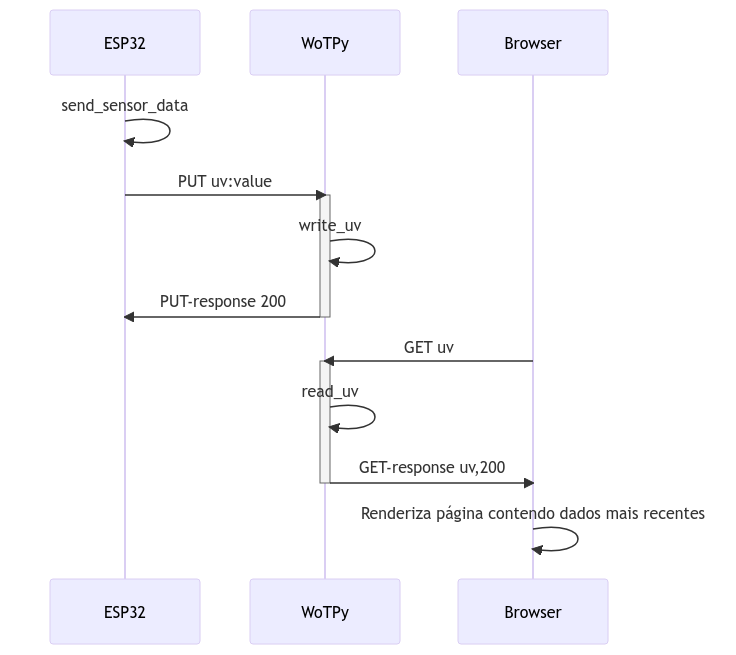
\includegraphics[scale=0.6]{figs/sequencia.png}
    \caption{O dispositivo (ESP32) executa um loop que, a cada 5 segundos executa a função send\_sensor\_data. Esta função envia uma requisição PUT para o servidor (WoTPy). Em resposta a essa requisição o servidor executa o handler (função) write\_uv que contém o envio da resposta. Um usuário pode acessar a informação no servidor através do Browser. Entrar a URL na barra de endereços do Browser o faz enviar ao servidor uma requisição GET. Em resposta à requisição o servidor executa o handler (função) read\_uv, que contém o envio da resposta - no caso, o valor de uv mais recente. O Browser recebe essa informação e renderiza a página contendo a informação.}
    \label{fig:sequencia}
\end{figure}

